% --- Slide 1: Abstract ---
\begin{frame}{Abstract}
    \begin{itemize}
        \item \textbf{Objective:} Implementation of a real-time executive capable of dynamic task activation via a distributed TCP/IP interface.
        \item \textbf{Core Problem:} Ensuring system determinism when task sets change at runtime.
        \item \textbf{Solution:} A multi-threaded server utilizing \textbf{Rate Monotonic Scheduling (RMS)} principles and \textbf{Response Time Analysis (RTA)} to validate schedulability before task admission.
        \item \textbf{Key Achievement:} A robust synchronization mechanism managing the tension between asynchronous network commands and synchronous periodic task execution.
    \end{itemize}
\end{frame}

% --- Slide 2: System Requirements & Constraints ---
\begin{frame}{System Requirements \& Constraints}
    The system simulates a real-time operating system (RTOS) environment:
    \begin{block}{Task Model}
        Each task $T_i$ is defined by a triplet $(C_i, P_i, D_i)$:
        \begin{itemize}
            \item $C_i$: Computation time (CPU usage).
            \item $P_i$: Periodicity.
            \item $D_i$: Deadline ($D_i \leq P_i$).
        \end{itemize}
    \end{block}
    \begin{block}{Operational Constraints}
        \begin{itemize}
            \item \textbf{Dynamic Admission:} Tasks are activated/deactivated via remote TCP commands.
            \item \textbf{Resource Limits:} A fixed capacity for active tasks ($N=4$) and thread limits for client connections.
            \item \textbf{Determinism:} Use of monotonic clocks to prevent drift and jitter.
        \end{itemize}
    \end{block}
\end{frame}

% --- Slide 3: Architectural Overview ---
\begin{frame}{High-Level Architecture}
    The system follows a three-tier hierarchical architecture:
    
    \begin{center}
        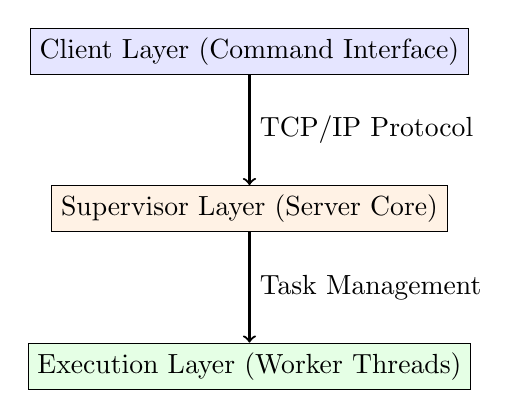
\begin{tikzpicture}[node distance=2cm]
            \node (client) [draw, rectangle, fill=blue!10] {Client Layer (Command Interface)};
            \node (server) [draw, rectangle, fill=orange!10, below of=client] {Supervisor Layer (Server Core)};
            \node (tasks) [draw, rectangle, fill=green!10, below of=server] {Execution Layer (Worker Threads)};
            
            \draw[->, thick] (client) -- (server) node[midway, right] {TCP/IP Protocol};
            \draw[->, thick] (server) -- (tasks) node[midway, right] {Task Management};
        \end{tikzpicture}
    \end{center}

    \begin{itemize}
        \item \textbf{Client Layer:} Parses user input and transmits encoded command payloads.
        \item \textbf{Supervisor Layer:} Manages the connection pool, handles command parsing, and performs schedulability checks.
        \item \textbf{Execution Layer:} Dedicated threads for periodic task routines using absolute time-based sleeping.
    \end{itemize}
\end{frame}

% --- Slide 4: Task Modeling Logic ---
\begin{frame}{Data Structures \& Task Modeling}
    To separate static definitions from runtime instances, we implement a dual-structure approach:

    \begin{columns}
        \begin{column}{0.5\textwidth}
            \textbf{Static: \texttt{Task}}
            \begin{itemize}
                \item \texttt{id}
                \item \texttt{cpu\_usage} ($C_i$)
                \item \texttt{period} ($P_i$)
                \item \texttt{deadline} ($D_i$)
                \item \texttt{routine} (Function Pointer)
            \end{itemize}
        \end{column}
        \begin{column}{0.5\textwidth}
            \textbf{Dynamic: \texttt{ActiveTask}}
            \begin{itemize}
                \item \texttt{task\_id} (Link to catalog)
                \item \texttt{instance\_id} (For instance tracking)
                \item \texttt{thread\_id} (Handle for lifecycle)
                \item \texttt{client\_port} (Ownership tracking)
            \end{itemize}
        \end{column}
    \end{columns}
    \vspace{0.5cm}
    The \texttt{TASK\_CATALOG} acts as the "Read-Only" truth, while \texttt{tasks\_active} represents the "Mutable" state of the system.
\end{frame}

% --- Slide 5: Schedulability Policy ---
\begin{frame}{Schedulability Policy: The Decision Engine}
    Before admitting a new task $T_{new}$, the system performs a hierarchical feasibility test:

    \begin{enumerate}
        \item \textbf{Utilization Factor Test (Necessary Condition):}
        Calculate total utilization $U$:
        \[ U = \sum_{i=1}^{n} \frac{C_i}{P_i} \leq 1.0 \]
        If $U > 1.0$, the task is rejected immediately.
        
        \item \textbf{Sufficient Condition Test (Liu \& Layland):}
        If $U \leq n(2^{1/n}-1)$, the system is guaranteed to be schedulable. In our implementation, we use the lower bound of $\ln(2) \approx 0.693$ for rapid verification.
        
        \item \textbf{Response Time Analysis (Exact Test):}
        If $0.693 < U \leq 1.0$, we proceed to the iterative RTA to determine if a deadline miss is possible.
    \end{enumerate}
\end{frame}

% --- Slide 6: Response Time Analysis (RTA) Implementation ---
\begin{frame}{Mathematical Logic: RTA Algorithm}
    The algorithm computes the worst-case response time $R_i$ for each task in the set.
    
    \begin{block}{The Iterative Equation}
        For each task $i$, we solve for $R_i$ using:
        \[ R_i^{(k+1)} = C_i + \sum_{j \in hp(i)} \left\lceil \frac{R_i^{(k)}}{P_j} \right\rceil C_j \]
        where $hp(i)$ is the set of higher-priority tasks.
    \end{block}

    \textbf{Implementation in \texttt{rta.c}:}
    \begin{itemize}
        \item \textbf{Sorting:} Tasks are sorted by period $P_i$ (Rate Monotonic Priority).
        \item \textbf{Convergence:} The loop continues until $R_i^{(k)} = R_i^{(k-1)}$.
        \item \textbf{Failure Condition:} If $R_i > D_i$, the task set is declared \textbf{unschedulable}.
    \end{itemize}
\end{frame}

% --- Slide 7: Concurrency Model & Threading ---
\begin{frame}{Concurrency Model: Threading Hierarchy}
    The system utilizes a dual-level threading model to ensure scalability and responsiveness:

    \begin{itemize}
        \item \textbf{Connection Management:}
        Each client connection is handled by a \texttt{connectionHandler} thread. This prevents a single slow client from blocking the server's ability to accept new connections.
        
        \item \textbf{Task Execution:}
        Once a task is admitted, a worker thread is spawned (\texttt{handling\_active\_task}).
        \begin{itemize}
            \item The thread executes the \texttt{routine()}.
            \item It uses \texttt{clock\_nanosleep(CLOCK\_MONOTONIC, ...)} to ensure precise periodic execution.
            \item It monitors the \texttt{active} flag to allow for graceful deactivation.
        \end{itemize}
    \end{itemize}
\end{frame}

% --- Slide 8: Synchronization & Data Integrity ---
\begin{frame}{Synchronization & Resource Management}
    To prevent race conditions in a multi-threaded, multi-client environment, several primitives are employed:

    \begin{description}
        \item[Mutexes] 
            \begin{itemize}
                \item \texttt{active\_tasks\_mutex}: Protects the \texttt{tasks\_active} array during addition, removal, and RTA analysis.
                \item \texttt{mutex} (Server): Protects the client connection buffer.
                \item \texttt{log\_mutex}: Ensures atomic, non-interleaved console output.
            \end{itemize}
        \item[Semaphores]
            \begin{itemize}
                \item \texttt{free\_slots\_sem}: A counting semaphore that limits the number of concurrent active tasks, preventing over-subscription of the task array.
            \end{itemize}
        \item[Condition Variables]
            \begin{itemize}
                \item \texttt{roomAvailable}: Manages client flow control, blocking new connections if the client buffer is full.
            \end{itemize}
    \end{description}
\end{frame}

% --- Slide 9: Implementation Details: Deterministic Timing ---
\begin{frame}{Implementation: Deterministic Timing Control}
    A critical component of a real-time executive is the ability to handle "next wake-up" calculations without cumulative error.

    \begin{exampleblock}{Absolute Time Calculation}
        Instead of relative sleeps (which accumulate drift), the system calculates the \textbf{Absolute Wake-up Time}:
        \begin{enumerate}
            \item Fetch current monotonic time.
            \item Calculate $T_{next} = T_{current} + P_i$.
            \item Use \texttt{clock\_nanosleep} with \texttt{TIMER\_ABSTIME}.
        \end{enumerate}
    \end{exampleblock}

    \textbf{Handling Nanosecond Overflows:}
    The code manually adjusts \texttt{tv\_sec} and \texttt{tv\_nsec} to handle the overflow where $nsec \ge 10^9$, ensuring the kernel receives a valid \texttt{timespec} structure.
\end{frame}

% --- Slide 10: Control Flow Summary ---
\begin{frame}{Command Processing Flow}
    \begin{center}
        \begin{tikzpicture}[scale=0.8]
            \node (start) [draw, circle] {Start};
            \node (recv) [draw, rectangle, below of=start] {Receive Command};
            \node (parse) [draw, diamond, below of=recv] {Parse Type};
            \node (sched) [draw, rectangle, below of=parse, xshift=2cm] {Schedulability Check};
            \node (act) [draw, rectangle, below of=sched] {Activate Thread};
            \node (deact) [draw, rectangle, below of=parse, xshift=-2cm] {Deactivate};
            \node (end) [draw, circle, below of=act] {End Loop};

            \draw[->] (start) -- (recv);
            \draw[->] (recv) -- (parse);
            \draw[->] (parse) -- node[above] {ACTIVATE} (sched);
            \draw[->] (parse) -- node[above] {BLOCK} (deact);
            \draw[->] (sched) -- (act);
            \draw[->] (act) -- (end);
            \draw[->] (deact) -- (end);
        \end{tikzpicture}
    \end{center}
    \begin{itemize}
        \item \textbf{Safety First:} The "Schedulability Check" is a mandatory gateway before "Activate Thread".
        \item \textbf{Graceful Exit:} The \texttt{STOP} command triggers a broadcast to all clients to ensure a synchronized shutdown.
    \end{itemize}
\end{frame}

% --- Slide 11: Conclusion ---
\begin{frame}{Conclusion}
    \begin{itemize}
        \item \textbf{Robustness:} The implementation successfully bridges high-level networking with low-level real-time scheduling requirements.
        \item \textbf{Mathematical Rigor:} By combining Utilization Bounds with RTA, the system provides $100\%$ accuracy in task admission decisions.
        \item \textbf{Scalability:} The use of thread-per-client and thread-per-task models allows for efficient resource utilization in a multi-core environment.
        \item \textbf{Future Work:}
            \begin{itemize}
                \item Implementation of Earliest Deadline First (EDF) scheduling.
                \item Support for multi-core task affinity.
                \item Enhanced jitter analysis.
            \end{itemize}
    \end{itemize}
    \vspace{0.5cm}
    \centering
    \textbf{Thank you for your attention. Questions?}
\end{frame}